% Part: model-theory
% Chapter: interpolation
% Section: separation

\documentclass[../../../include/open-logic-section]{subfiles}

\begin{document}

\olfileid{mod}{int}{sep}

\olsection{\printtoken{P}{sentence}-এর পৃথকীকরণ}

ইন্টারপোলেশন উপপাদ্যের প্রমাণে এগোনোর আগে কিছু প্রাথমিক কাজ দরকার।
$!A$ ও $!B$-এর একটি ইন্টারপোল্যান্ট হলো এমন একটি !!a{sentence}~$!C$ যাতে
$!A \Entails !C$ এবং $!C \Entails !B$। বিপরীতকরণ অনুসারে, শেষের
বক্তব্যটি সত্য হওয়ার সমতুল্য হলো $\lnot !B \Entails \lnot !C$।
এই বৈশিষ্ট্যযুক্ত !!^a{sentence}~$!C$-কে $!A$ ও $\lnot !B$-কে
\emph{পৃথক করে} বলা হয়। অতএব $!A$ ও $!B$-এর একটি ইন্টারপোল্যান্ট খোঁজা
মানে এমন একটি !!a{sentence} খোঁজা, যা $!A$ ও $\lnot !B$-কে পৃথক করে।
যেমন প্রায়ই হয়, আরও সাধারণ রূপটি বিবেচনা করা সুবিধাজনক: দুটি
!!{sentence}s-এর \emph{সমষ্টি}-কে পৃথক করে এমন একটি বাক্য।

\begin{defn}
দুটি বাক্যের সমষ্টি $\Gamma$ এবং $\Delta$-কে একটি বাক্য $!C$
\emph{পৃথক করে} যদি এবং কেবল যদি $\Gamma \Entails !C$ এবং
$\Delta \Entails \lnot !C$। এমন কোনো !!{sentence} না থাকলে
$\Gamma$ ও $\Delta$-কে \emph{অপৃথকযোগ্য} বলা হয়।
\end{defn}

$\Gamma$, $\Delta$ এবং $!C$-এর মডেলের শ্রেণির অন্তর্ভুক্তি-সম্পর্ক
নিচে দেখানো হলো:
\begin{figure}[h]
  \centering
  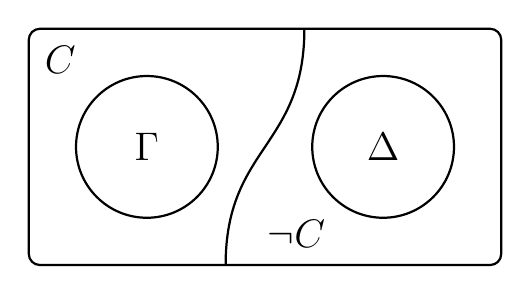
\begin{tikzpicture}[node distance=2cm, auto, thick]
    \draw [rounded corners] (0,0) -- (6,0) -- (6,3) -- (0,3) --  cycle;
    \draw (1.5,1.5) circle (0.9cm);
    \draw (4.5,1.5) circle (0.9cm);
    \path node at (1.5,1.5) {\Large $\Gamma$};
    \path node at (4.5,1.5) {\Large $\Delta$};
    \path node at (0.4,2.6) {\Large $\formula{C}$};
    \path node at (3.4,0.4) {\Large $\lnot \formula{C}$};
    \draw (2.5,0) .. controls (2.5,1.5) and (3.5,1.5) .. (3.5,3);
  \end{tikzpicture}
  \caption{$!C$ $\Gamma$ ও $\Delta$-কে পৃথক করে}
  \ollabel{fig:sep}
\end{figure}


\begin{lem}\ollabel{lem:sep1}
ধরা যাক, $\Lang{L}_0$ হলো এমন ভাষা যাতে $\doteq$ ছাড়া
$\Gamma$ ও $\Delta$ উভয়টিতে ঘটে এমন প্রতিটি !!{constant}s,
!!{function} এবং !!{predicate} আছে, এবং $\Lang{L}'_0$ পাওয়া যায়
$n \ge 0$-এর জন্য অসীমসংখ্যক নতুন !!{constant} $\Obj c_n$ যোগ করে।
তাহলে $\Lang{L}_0$-তে $\Gamma$ ও $\Delta$ অপৃথকযোগ্য হলে
$\Lang{L}'_0$-তেও তারা অপৃথকযোগ্য।
\end{lem}

\begin{proof}
বিপরীত ধরে এগোই: ধরা যাক $\Lang{L}'_0$-তে $\Gamma$ ও $\Delta$
পৃথকযোগ্য। তাহলে $!C \in \Lang{L}_0$-এর জন্য
$\Gamma \Entails \Subst{!C}{c}{x}$ এবং
$\Delta \Entails \lnot \Subst{!C}{c}{x}$, যেখানে $c$ একটি নতুন
!!{constant} (এখানে $!C$-তে একাধিক এমন নতুন !!{constant} থাকলে একই
যুক্তি প্রযোজ্য)। সংহতি থেকে $\Gamma$-এর একটি \emph{সসীম}
উপসেট $\Gamma_0$ এবং $\Delta$-এর একটি সসীম উপসেট $\Delta_0$ আছে,
যাতে $\Gamma_0 \Entails \Subst{!C}{c}{x}$ এবং
$\Delta_0 \Entails \lnot \Subst{!C}{c}{x}$। $\Gamma_0$-এর
সব !!{formula}s-এর সংযোজনকে $!G$ এবং $\Delta_0$-এর সব !!{formula}s-এর
সংযোজনকে $!H$ ধরি। তাহলে
\begin{align*}
  !G & \Entails \Subst{!C}{c}{x}, & !H  \Entails \lnot \Subst{!C}{c}{x}.
\end{align*}
প্রথমটি থেকে সাধারণীকরণের সাহায্যে $!G \Entails \lforall[x][!C]$
পাই, আর দ্বিতীয়টি থেকে বিপরীতকরণের সাহায্যে
$\Subst{!C}{c}{x} \Entails \lnot !H$; অতএব
$\lforall[x][!C] \Entails \lnot !H$। আবার বিপরীতকরণে
$!H \Entails \lnot \lforall[x][!C]$। একঘেয়েমি সূত্রে,
\begin{align*}
  \Gamma & \Entails \lforall[x][!C], &
  \Delta & \Entails \lnot \lforall[x][!C],
\end{align*}
ফলে $\lforall[x][!C]$ $\Lang{L}_0$-তে $\Gamma$ ও $\Delta$-কে
পৃথক করে। এটি বিরোধ।
% BN-SRC-134 TARGET-CORRECTION-BEGIN
\par\smallskip\noindent\textnormal{\small\textbf{উৎস-সংশোধন (BN-SRC-134):} হিমায়িত প্রমাণে উপরোক্ত সর্বজনীকৃত সূত্রের পরিণতি হিসেবে ভুলভাবে $\lnot \delta$ লেখা আছে। সেখানে একই লাইনে সংজ্ঞায়িত $!H$-ই উদ্দেশ্য; বাংলা সূত্রে $\lnot !H$ পুনরুদ্ধার করা হয়েছে।} % BN-SRC-134 TARGET-CORRECTION-END
\end{proof}

\begin{lem}\ollabel{lem:sep2}
ধরা যাক $\Gamma \cup \{ \lexists[x][!S] \}$ এবং $\Delta$
অপৃথকযোগ্য, এবং $c$ হলো $\Gamma$, $\Delta$ বা $!S$-এ নেই এমন
একটি নতুন !!{constant}। তাহলে $\Gamma \cup \{
\lexists[x][!S], \Subst{!S}{c}{x} \}$ এবং $\Delta$-ও
অপৃথকযোগ্য।
\end{lem}

\begin{proof}
বিরোধের জন্য ধরি, $!C$ $\Gamma \cup \{
\lexists[x][!S], \Subst{!S}{c}{x}\}$ এবং $\Delta$-কে পৃথক করে,
যদিও $\Gamma \cup \{\lexists[x][!S] \}$ ও $\Delta$
অপৃথকযোগ্য। দুটি ঘটনা আলাদা করি:
\begin{enumerate}
\item $c$ যদি $!C$-তে না থাকে, তবে
  $\Gamma \cup \{\lexists[x][!S], \lnot!C \}$ সন্তোষণীয়
  (নইলে $!C$ $\Gamma \cup \{\lexists[x][!S] \}$ ও $\Delta$-কে
  পৃথক করত)। $\Subst{!S}{c}{x}$ যোগ করলেও এটি সন্তোষণীয় থাকে, তাই
  শেষ পর্যন্ত $!C$ $\Gamma \cup \{ \lexists[x][!S],
  \Subst{!S}{c}{x} \}$ ও $\Delta$-কে পৃথক করে না।
\item $c$ যদি $!C$-তে থাকে, তবে $!C$-এর রূপ
  $\Subst{!C}{c}{x}$। সুতরাং
   \[
  \Gamma \cup \{ \lexists[x][!S], \Subst{!S}{c}{x}\} \Entails \Subst{!C}{c}{x},
   \]
  এবং নিঃসরণ উপপাদ্য ও সাধারণীকরণে
  $\Gamma, \lexists[x][!S] \Entails \lforall[x][(!S \lif !C)]$;
  শেষে $\Gamma \cup \{ \lexists[x][!S] \} \Entails
  \lexists[x][!C]$। অন্যদিকে
  $\Delta \Entails \lnot \Subst{!C}{c}{x}$, তাই সাধারণীকরণে
  $\Delta \Entails \lnot \lexists[x][!C]$। ফলে
  $\Gamma \cup \{\lexists[x][!S] \}$ ও $\Delta$ পৃথকযোগ্য—বিরোধ।
\end{enumerate}
% BN-SRC-135 TARGET-CORRECTION-BEGIN
\par\smallskip\noindent\textnormal{\small\textbf{উৎস-সংশোধন (BN-SRC-135):} হিমায়িত পাঠে এই অনুমানের এক জায়গায় $\lexists[x]{!S}$-এ দ্বিতীয় জোড়া বন্ধনী অনুপস্থিত। বাংলা সূত্রে একই সংজ্ঞার সঠিক $\lexists[x][!S]$ রূপ সর্বত্র রাখা হয়েছে।} % BN-SRC-135 TARGET-CORRECTION-END
\end{proof}

\end{document}
